\chapter{Kinetics}
\section{Introduction}
\subsection{Topics}
\begin{enumerate}
  \item Definition of Rate
  \item Related rates and stoichiometry
  \item Rates and KMT
  \item Reaction Order
  \item Temperature and rate
  \item Mechanisms of reaction
\end{enumerate}

\section{Rates and Reactions}
To illustrate the rates for a simple reaction, an example is shown:

\ce{2NO2(g) -> N2O4(g)}

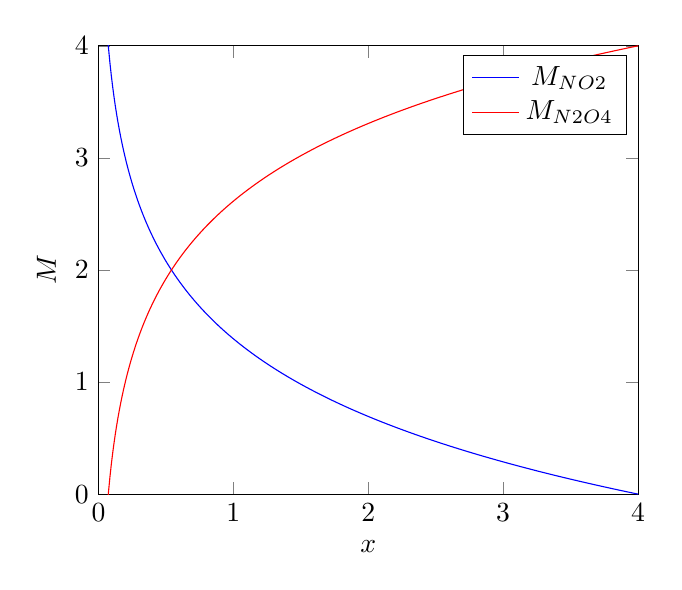
\begin{tikzpicture}
  \begin{axis}[
      xlabel=$x$, ylabel=$M$,
      xmin=0, xmax=4,
      ymin=0, ymax=4,
      legend entries={$M_{\ce{NO2}}$, $M_{\ce{N2O4}}$}
    ]
    \addplot[blue, samples=1000] {-ln(x/4)};
    \addplot[red, samples=1000] {ln(x/4)+4};
  \end{axis}
\end{tikzpicture}

\begin{equation}
  \frac{d}{dt}\left[\ce{N2O4}\right] = \frac{-1}{2}\frac{d}{dt}\left[\ce{NO2}\right]
\end{equation}

Rates are given to have coefficients of the inverse of their stoichiometric
coefficient, and have a negative sign only if they are a reactant.

\section{Changing the Reaction Rate}
On a molecular level, the following occur during a reaction:
\begin{enumerate}
  \item Reacting particles must come into contact with each other.
  \item The particles must have some amount of energy available to break
    existing bonds.
  \item The orientntation of the reacting species may be important in the
    reacting process.
\end{enumerate}

As such, the rate at which a reaction occurs may be altered in the following
ways:
\begin{description}
  \item[Change the concentration of the reactants] The concentration of the
    reactants is directly proportional to the amount of times the reacting
    species will come into contact with each other.
  \item[Temperature] temperature not only determines molecular speed but also
    the amount of energy available to break bonds. If we increase temperature,
    not only will we get more collisions, but we'll have more collisions that
    break bonds.
  \item[Catalysts] A catalyst is a substance that is not used up in the
    reaction, but fits with the reacting species as a "key" to orient them
    together to react more effectively.
\end{description}

\section{Rate Law}
\begin{equation}
  \text{rate}=k[R_1]^m[R_2]^n \ldots
\end{equation}

To calculate the rate law for an equation involving two products, you must
eliminate all exponents except for one and then solve. Once that information is
obtained, you can go back, determine the other exponent, and then the value of
$k$. An example is shown below:\\

\textit{Both A and B are reactants. We look at the rate of reaction in several
different experiments.}

\begin{table}[]
\centering
\begin{tabular}{l|l|l|l|}
\cline{2-4}
                        & {[}A{]} & {[}B{]} & Initial rate (M/sec) \\ \hline
\multicolumn{1}{|l|}{1} & 0.1     & 0.1     & 0.014                \\ \hline
\multicolumn{1}{|l|}{2} & 0.1     & 0.2     & 0.056                \\ \hline
\multicolumn{1}{|l|}{3} & 0.5     & 0.2     & 0.280                \\ \hline
\multicolumn{1}{|l|}{4} & 1.0     & 0.4     & 2.24                 \\ \hline
\end{tabular}
\end{table}

\begin{equation}
  \begin{split}
    \frac{\SI{.056}{\Molar\per\second}}{\SI{.014}{\Molar\per\second}} &=
    \frac{k[0.1]^m[0.2]^n}{k[0.1]^m[0.1]^n}\\
    4 &= 2^n \Rightarrow n = 2
  \end{split}
\end{equation}

\begin{equation}
  \begin{split}
    \frac{\SI{.280}{\Molar\per\second}}{\SI{.056}{\Molar\per\second}} &=
    \frac{k[0.5]^m[0.2]^n}{k[0.1]^m[0.2]^n}\\
    5 &= 5^m \Rightarrow m = 5
  \end{split}
\end{equation}

\begin{equation}
  \SI{.014}{\Molar\per\second}=k[0.1][0.1]^2\\
  k=\SI{14}{\Molar\squared\per\second}
\end{equation}

\section{First Order Reactions}
First order reactions proceed according to one reactant. We know, therefore,
that the following is true:

\begin{equation}
  \text{rate}=k[R]^1
\end{equation}

Therefore...

\begin{equation}
  \begin{split}
    \text{rate} &= \frac{-d[R]}{dt}\\
                &= k[R]
  \end{split}
\end{equation}

\begin{equation}
  \frac{1}{[R]}d[R]=-k dt
\end{equation}

\begin{equation}
  \int_{[R]_0}^{[R]_t} \frac{1}{[R]} d[R] = -k\int_{0}^{1} dt
\end{equation}

Which yields the integrated rate-law (1st order):

\begin{equation}
  \ln([R]_t) - \ln([R]_0) = -kt
\end{equation}

This produces a graph which looks like the following:

\begin{tikzpicture}
  \begin{axis}[
    xlabel={$t$}, ylabel={$\ln[A]$},
     xmin=0, xmax=5
  ]

    \addplot[blue] {-x};
  \end{axis}
\end{tikzpicture}

\subsection{$n^{\text{th}}$-life}
To calculate the $n^{\text{th}}$ life of a reactant, you simply use the
integrated rate law and the following equation:

\begin{equation}
  \frac{[R]_1}{[R]_0} = \frac{1}{n}
\end{equation}
